\documentclass{article}
\usepackage[utf8]{inputenc}

\title{Deep Networks: ImageNet}
\author{Mihir Patel}
\date{November 2017}

\usepackage{natbib}
\usepackage{graphicx}
\usepackage{amsmath}

\begin{document}

\maketitle

\section{Introduction}
One of the greatest problems in AI has been in working with images and visual input. As we learned before, convolutional neural networks are very effective at doing this. One of the great challenges that has pushed this field forward is ImageNet. ImageNet is a classification challenge where 1 million images are given and must be classified. Many groups all over the world strive to improve modern AI technology in order to top the charts annually. In order to produce more succesful results, many optimizations have been done to the standard neural network.

\section{Softmax}
\begin{center}
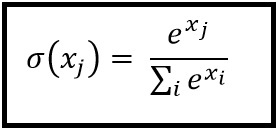
\includegraphics[scale=0.5]{softmax}
\end{center}
\subsection{Definition}
The first challenge in this is how we can optimize determining which class something is. At the end of the network, we have one neuron per each output class (say 2 with dog and cat). We want to know which output class the image is. In simple cases, you can just take the highest. However, ImageNet allows you to take your top 5 best guesses since many classes turn out to be similar with thousands of classes (say different breeds of dogs). We want a way to estimate the probability of each label. To do this, we use the softmax layer. This function essentially takes the sum of all the outputs and raises it to e to make it positive. It then calculates the probability of each label by taking its value raised to e over the total sum just calculated, which essentially shows us how much of the sum it consists of, nicely giving us a probability.

\section{VGG16}
\begin{center}
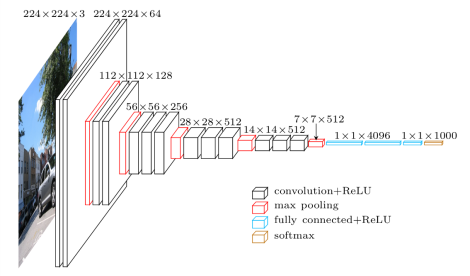
\includegraphics[scale=0.5]{vgg16}
\end{center}
\subsection{Definition}
One of the first networks that performed well combining all this so far was vgg16. This network was able to classify images across thousands of categories with 90 percent accuracy given top 5 class guesses and 70.5 percent with top 1. This structure is still commonly used for many modern problems and has the benefits of being simple and easy to train. It has a slightly more powerful older cousin called vgg19 which is also very popular.

\section{Residual Connections}
\begin{center}
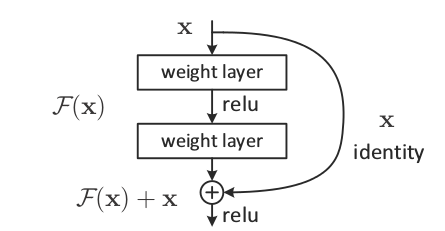
\includegraphics[scale=0.5]{resnet}
\end{center}
\subsection{Definition}
For some years, the trend in machine learning was always adding more layers. With the constant improvement in GPUs, if something didn't work now, the solution was to wait a year and add more layers. However, one big issue that exists with this is the vanishing gradient. At some point, the connection between the input and the output is too spaced away and the network can no longer learn significant features at the lower layers. However, we know that deeper networks can learn more complex features more easily and are much better suited to handle hard problems. To solve this, researchers produced residual connections. Residual connections are essentially these nodes which consist of a set of layers. Each node extracts some features from the raw image and then combines this information with the original input to pass into the subsequent layer. In this way, features can be extracted in depth and subsequent layers can maintain access to the original information. 

\section{ResNet}
\begin{center}
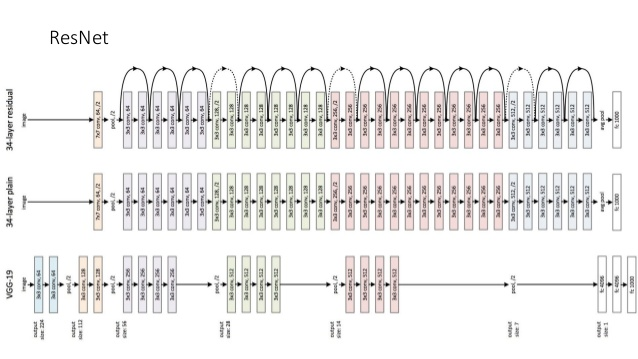
\includegraphics[scale=0.5]{resnet.jpg}
\end{center}
\subsection{Definition}
As you can see, ResNet allows for much greater depth compared to VGG. This, too, is the smallest size of ResNet. Typical applications use ResNet-50 at least and high-end ones use ResNet-152. The sheer power of these structures has allowed for 92.9 percent accuracy on ImageNet and the usage of training on fancy GPUs with lots of data.

\section{Inception}
\begin{center}
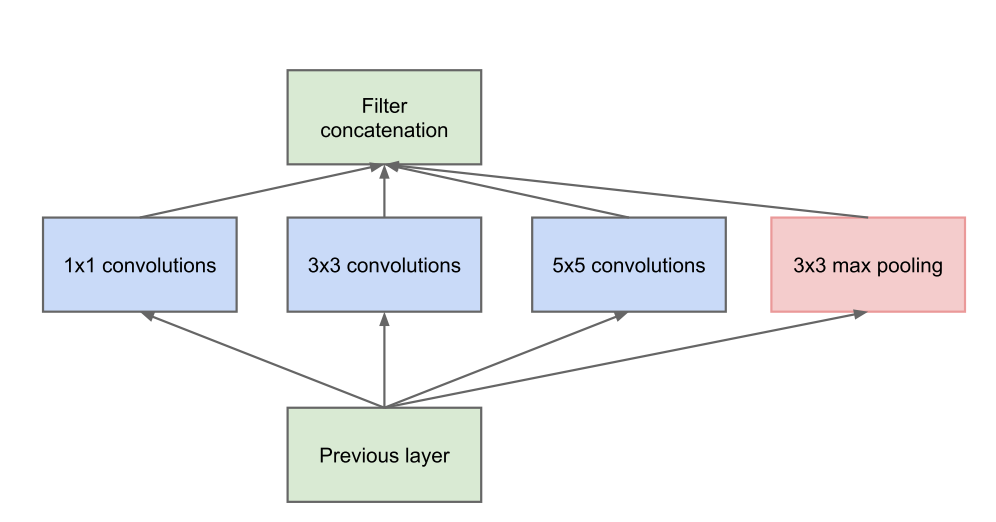
\includegraphics[scale=0.5]{inception}
\end{center}
\subsection{Definition}
The last major improvement in recent years in image classification has been in the usage of multiple parallel layers in each residual node. Each of these sets of layers, as seen in the image above, contains different filter sizes, allowing for a varying size of features to be extracted. From this, each residual node can learn much more and increased information can be packed in. This has culminated in Inception-ResNet structures capable of producing results more accurate than humans on image classification.

\section{To the Future}
In large part, following these advances, image classification has been solved. Without massive amounts of data, performance enhancements will largely be negligible. However, as these structures have gotten bigger, they have also gotten slower and slower. In recent years, the next step has been in breaking down multiple objects and analyzing complex images.

\end{document}
